\documentclass[a4,9pt]{beamer}
\usetheme{Singapore}
\usepackage{multicol}
\usepackage{xcolor}
\usepackage{graphicx}
\linespread{1.35}
\usepackage{amsmath}
\usepackage{color}
\usepackage{tikz}
\usetikzlibrary{arrows,automata}

\begin{document}
\begin{frame}
\section*{Finite State Machine}
\begin{flushright}
\texttt{Finite State Machine} \hspace*{0.1cm}\textbf{$|$} \hspace*{0.1cm} \textbf{177}\hspace*{0.1cm}
\end{flushright}
\vspace*{1cm}

\large{\textbf{Solution:}}

\pause
\begin{center}
\begin{tabular}{ccc}
 \hline

 \hline

 \hline

 \hline
 & \multicolumn{2}{c}{Next State,Z}\\
 \cline{2-3}
Present State & X=0           &   X=1\\
\hline
    A    &  A,0  & B,0 \\
    B    &  C,0  & D,0 \\
    C    &  D,1  & C,1 \\
    D    &  B,1  & A,1 \\
 \hline

 \hline

 \hline

 \hline
\end{tabular}
\end{center}

\pause
First, we need to prove whether the machine is information lossless. For this, we need to construct a testing table for information lossless.
\end{frame}

\begin{frame}

\begin{center}
  \begin{tabular}{ccc}
\hline

\hline

\hline

\hline
Present State & z = 0 & z = 1\\
\hline
 A &     AB    &     --      \\
 B &     CD    &     --      \\
 C &     --    &     CD      \\
 D &     --    &     AB      \\
\hline
AB & (AC)(BC)  &     --      \\
   & (AD)(BD)  &             \\
CD &   --      &  (BD)(BC)   \\
   &           &  (AD)(AC)   \\
AC &   --      &     --      \\
AD &   --      &     --      \\
BC &   --      &     --      \\
BD &   --      &     --      \\
\hline

\hline

\hline

\hline

  \end{tabular}
\end{center}

\pause
The testing table does not contain any repeated entry. So, the machine is information lossless. Now, we need to construct the output successor table

\end{frame}

\begin{frame}

 \begin{flushleft}
    \textbf{178}\hspace*{0.1cm} \textbf{$|$} \hspace*{0.1cm} {\tiny \textbf{Introduction to Automata Theory, Formal Languages and Computation}}
  \end{flushleft}
\section*{Introduction to Automata Theory, Formal Languages and Computation}
\vspace*{0.1cm}

\section{picture}
\includegraphics[width=15cm,height=12cm]{نمودار سحر.png}

\end{frame}

\begin{frame}

After traversing the total output string by the output successor table, we have got a state B. So, the input string is 01000.(Input string retrieval is possible only for an information lossless machine. This can be illustrated in the following example.)

\pause
\vspace*{0.3cm}
\fcolorbox{red}{yellow}{\textcolor{blue}{Example 4.20}} \hspace*{0.2cm} \footnotesize{Convert the given Mealy machine to an equivalent Moore machine.}

\vspace*{0.3cm}
\pause
\large{\textbf{Solution:}}
\vspace*{0.2cm}

\pause
\begin{center}
\begin{tabular}{ccc}
\hline

\hline

\hline

\hline
  \multicolumn{3}{r}{{Next State,Z}}\\
 \cline{2-3}
{Present State} & {X=0} & {X=1}\\
\hline
 A & B,0 & B,0 \\
 B & C,0 & D,0\\
 C & D,0 & C,0\\
 D & A,0 & C,1\\
\hline

\hline

\hline

\hline
\end{tabular}
\end{center}
\end{frame}

\begin{frame}
 The machine is not information lossless as, in the testing table, for information losslessness, there
is a repeated entry BB for the state ‘A’ and output ‘0’. Yet, again we try to fi nd the input sequence by
constructing the output successor table.
\end{frame}

\begin{frame}
\section*{Finite State Machine}
\begin{flushright}
\texttt{Finite State Machine} \hspace*{0.1cm}\textbf{$|$} \hspace*{0.1cm} \textbf{179}\hspace*{0.1cm}
\end{flushright}
\vspace*{1cm}

The output successor table for the given machine is

\pause
\begin{center}
\begin{tabular}{ccc}
\hline

\hline

\hline

\hline
  \multicolumn{3}{r}{{Next State,Z}}\\
 \cline{2-3}
{Present State} & {Z=0} & {Z=1}\\
\hline
 A & B/0,B/1 & -- \\
 B & D/0,D/1 & -- \\
 C & D/0,C/1 & -- \\
 D &  A/0    & C/1\\
\hline

\hline

\hline

\hline
\end{tabular}
\end{center}

\pause
The input string is applied on the state A and has produced output 0. From the output successor table, it is clear that the next states are B with input 0 or B with input 1.
\end{frame}

\begin{frame}
By this process, the transition is given in Fig.4.27.
\pause
\section{picture}
\includegraphics[width=15cm,height=12cm]{نمودار  سحری.png}

\end{frame}

\begin{frame}
We are getting C as the final state for two input sequences 01101 and 11101. So, we cannot uniquely determine the input string. We can conclude that input string retrieval is not possible for the information lossy machine.

\pause
\vspace*{1cm}
\fcolorbox{red}{yellow}{\textcolor{blue}{Example 4.21}} \hspace*{0.2cm} Test whether the following machine is information lossless or not. If lossless, find its order.
\end{frame}

\begin{frame}

\begin{flushleft}
    \textbf{180}\hspace*{0.1cm} \textbf{$|$} \hspace*{0.1cm} {\tiny \textbf{Introduction to Automata Theory, Formal Languages and Computation}}
  \end{flushleft}
\section*{Introduction to Automata Theory, Formal Languages and Computation}

\vspace*{0.1cm}
\pause
\large{\textbf{Solution:}}

\pause
\begin{center}
\begin{tabular}{ccc}
\hline

\hline

\hline

\hline
  \multicolumn{3}{r}{{Next State,Z}}\\
 \cline{2-3}
{Present State} & {X=0} & {X=1}\\
\hline
 A & B,0 & C,0 \\
 B & D,0 & E,1 \\
 C & A,1 & E,0 \\
 D & E,0 & D,0 \\
 E & A,1 & E,1 \\
\hline

\hline

\hline

\hline
\end{tabular}
\end{center}

\pause
The first step to test whether a machine is lossless or not is to construct a testing table. The testing table is divided into two halves.
\end{frame}

\begin{frame}

\begin{center}
  \begin{tabular}{ccc}
\hline

\hline

\hline

\hline
Present State & z = 0 & z = 1\\
\hline
 A &     BC    &     --      \\
 B &     D     &     E      \\
 C &     E     &     A      \\
 D &     DE    &     --      \\
 E &     --    &     AE      \\
\hline
BD &   DE      &     AE      \\
DE &   --      &     --      \\
AE &   --      &     --      \\
\hline

\hline

\hline

\hline

  \end{tabular}
\end{center}

\pause
The testing table does not contain any repeated entry. The machine is an information lossless machine.
The testing graph for the machine is given in Fig. 4.28.

\end{frame}

\begin{frame}

\begin{center}
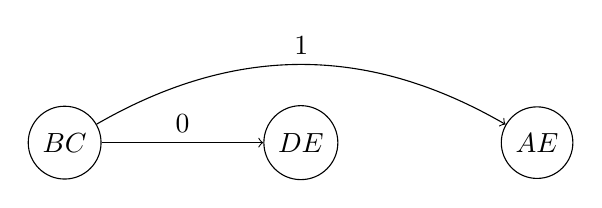
\begin{tikzpicture}[->,node distance = 3cm,auto]
  \node[state] (A) {$BC$};
  \node[state] (B) [right of=A] {$DE$};
  \path (A) edge node {$0$}(B);
  \node[state] (C) [right of = B] {$AE$};
  \path (A) edge [bend left] node {$1$}(C);
\end{tikzpicture}
\end{center}

\centerline{\textbf{Fig. 4.28}\hspace*{0.1cm} Testing Graph for Information Losslessness}
\vspace*{0.1cm}

The testing graph for information losslessness is loop-free. The order of losslessness is $m = 1 + 2 = 3$. The length of the longest path of the graph is $1$.
\vspace*{0.1cm}

\LARGE{\textbf{4.11 \hspace*{0.1cm} Inverse Machine}}
\vspace*{0.1cm}

\small{An inverse machine Mi is a machine which is developed from the given machine M with its output sequence and produces the input sequence given to machine M, after at most a fi nite delay.
A deterministic inverse machine can be constructed if and only if the given machine is lossless. The machine can produce the input sequence applied to the original machine after at most a fi nite delay if and only if M is lossless of a fi nite order. Consider the following example.}
\end{frame}

\end{document} 